\documentclass[a4paper]{article}
% Pacotes necessários
\usepackage[portuguese]{babel}
\usepackage[backend=biber, style=apa, citestyle=apa, language=portuguese]{biblatex}
\usepackage{csquotes}
\addbibresource{Recursos/referencias.bib}

\usepackage{amsmath}
\usepackage{graphicx}
\usepackage{subcaption}
\usepackage{setspace}
\usepackage{siunitx} % Required for alignment
\sisetup{
  round-mode          = places, % Rounds numbers
  round-precision     = 2, % to 2 places
}
\usepackage{enumerate}
\usepackage{enumitem}
\usepackage{amsmath}
\usepackage{karnaugh-map}
\usepackage[section]{placeins}
\usepackage{geometry}
\usepackage{amssymb}
\usepackage{titling}
\usepackage[T1]{fontenc}
\usepackage{float}
\usepackage[hidelinks]{hyperref}
\usepackage{xcolor}
\usepackage{indentfirst}
\usepackage{array}
\usepackage{soul}
\usepackage{afterpage}
\newcolumntype{P}[1]{>{\centering\arraybackslash}p{#1}}

% Comando para criar uma página vazia
\newcommand\myemptypage{
    \null
    \thispagestyle{empty}
    \addtocounter{page}{-1}
    \newpage
}

% Página de título principal
\newcommand{\firsttitlepage}{
    \begin{titlepage}
        \centering
        \vspace*{1cm}
        
        % Logos superior
        \begin{figure}[h!]
            \centering
            
\includegraphics[width=6cm]{Recursos/LOGO_IPB} % Substitua pelo caminho da imagem
            \vspace{0.5cm}
        \end{figure}

        % Informações da instituição
        \large\textbf{INSTITUTO POLITÉCNICO DE BEJA} \\
        \large\textbf{Escola Superior de Tecnologia e Gestão} \\
        \large\textbf{Licenciatura em Engenharia Informática} \\
        \large\textbf{Sistemas de Informação} \\
        
        \vspace{2cm}
        
        % Título do projeto
        {\Huge \textbf{Trabalho de Grupo 1}} \\
        
        \vspace{1.5cm}
        
        % Autores
        \large Martinho José Novo Caeiro - 23917 \\
        \large Paulo António Tavares Abade - 23919 \\
        
        \vfill
        
        % Logo inferior
        \begin{figure}[h!]
            \centering
            
\includegraphics[width=6cm]{Recursos/IPBejaESTIG.jpg} % Substitua pelo caminho da imagem
        \end{figure}
        
        \vspace{1cm}
        
        % Local e data
        {\large Beja, novembro de 2024}
    \end{titlepage}
}

\newcommand{\secondtitlepage}{
    \begin{titlepage}
        \centering
        \vspace*{1cm}
        
        % Informações da instituição
        \large\textbf{INSTITUTO POLITÉCNICO DE BEJA} \\
        \large\textbf{Escola Superior de Tecnologia e Gestão} \\
        \large\textbf{Licenciatura em Engenharia Informática} \\
        \large\textbf{Sistemas de Informação} \\
        
        \vspace{2cm}
        
        % Título do projeto
        {\Huge \textbf{Trabalho de Grupo 1}} \\
        
        \vspace{1.5cm}
        
        % Autores
        \large Martinho José Novo Caeiro - 23917 \\
        \large Paulo António Tavares Abade - 23919 \\

        \vspace{2cm}

        % Orientador
        \large Orientador: Professora Isabel Sofia Brito \\
        
        \vfill
        
        % Local e data
        {\large Beja, novembro de 2024}
    \end{titlepage}
}

\begin{document}
\pagenumbering{gobble} % Oculta numeração da página

% Primeira página de título
\firsttitlepage

\secondtitlepage
\renewcommand{\contentsname}{Índice}       % Título do sumário
\renewcommand{\listfigurename}{Índice de Figuras} % Título da lista de figuras

% Início do conteúdo do relatório
\newpage
\doublespacing
\tableofcontents
\listoffigures
\doublespacing

\newpage
\pagenumbering{arabic}

\section{Introdução}\label{intro}
Neste trabalho irá ser abordado como a Crise do Petróleo influenciou a produção e desenvolvimento
dos carros entre os anos 1970 e 1980, alterando o motor e por consequência a sua aceleração, eficiência e consumo.

Para analisar esta situação foi utilizada uma base de dados com 393 entradas, com 9 atributos iniciais, sendo estes:
 Milha por Galão, Cilindros, Cilindrada, Cavalagem, Peso, Aceleração, Ano de Fabrico, País de Origem e o Nome Completo do Carro.

Ainda foi utilizada outra base de dados que indica o preço médio de combustível por ano, entre 1970 e 1982, 
nos Estados Unidos da América.

Por fim, a nossa teoria é que a Crise do Petróleo influenciou a produção e 
desenvolvimento dos carros entre os anos 1970 e 1980, alterando o motor e por consequência a sua aceleração, eficiência e consumo.
%---------------------------------------------------------------------------------------------------------------------------
\section{Metodologia de Trabalho}\label{met}
Para o desenvolvimento deste trabalho foi utilizado o \textit{Github} para a partilha de código e documentação,
o \textit{Visual Studio Code} como IDE de desenvolvimento, o \textit{Excel - PowerQuery} ferramenta principal de tratamento
e análise de dados e por fim, o \textit{SQL Server Management} para a criação da Data Warehouse. 
%---------------------------------------------------------------------------------------------------------------------------
\section{ETL}\label{etl}
O trabalho de ETL foi realizado em 3 fases, a primeira foi a extração dos dados, 
a segunda a transformação e por fim a inserção dos dados em tabelas dinâmicas.
%---------------------------------------------------------------------------------------------------------------------------
\subsection{Extração de Dados}
Os dados foram extraídos de um ficheiro \textit{.csv} que foi encontrado no Kaggle (\cite{kaggle}) e no US Department of Energy (\cite{usdoe}), 
estes foram importados para o \textit{Excel} utilizando o PowerQuery. Foram ambos importados para o Excel e unidos numa única tabela.
%---------------------------------------------------------------------------------------------------------------------------
\subsection{Transformação de Dados}
Com o auxílio do PowerQuery foi possível transformar os dados, e foram encontrados diversos problemas,
como por exemplo, a presença de valores nulos, duplicados e a necessidade de alterar o tipo de dados de algumas colunas.
Ainda foram encontrados problemas com a formatação dos dados, como por exemplo, a presença de vírgulas em vez de pontos. 
Estes erros ocorreram nas colunas de: Milhas por Galão, Cilindros, Cavalagem, Aceleração e Preço da Gasolina.
Para resolver estes problemas foi necessário alterar o tipo de dados das colunas, remover os valores nulos e duplicados e substituir as vírgulas por pontos.
Existia alguns nomes com sinónimos, como por exemplo, "Chevrolet" e "Chevy", "Volkswagen" e "VW", "Datsun" e "Nissan", e alguns até mesmo mal escritos, 
como por exemplo, "Volkswagen" e "Vokswagen" ou "Mazda" e "Maxda".
Foi necessário transformar quase todos os campos para o tipo de dados correto, como por exemplo, a cavalagem para inteiro, 
a aceleração para decimal e o preço da gasolina para decimal.
As colunas originais eram: Nome, Milhas por Galão, Cilindros, Cilindrada, Cavalagem, Peso, Aceleração, Ano de Fabrico e País de Origem.
O nome das colunas também foi alterado para facilitar a sua identificação e foram adicionadas novas colunas para facilitar a análise
e permitir a criação de tabelas dinâmicas, sendo que as novas colunas são: Marca, Modelo e Preço da Gasolina.

\subsection{Visualização de Dados}
Utilizando as tabelas dinâmicas do Excel, foi possível visualizar os dados de forma mais clara e objetiva,
para isso, foram utilizados gráficos dinâmicos onde é possível visualizar a evolução dos carros ao longo dos anos,
a evolução da eficiência dos carros ao longo dos anos e ainda a evolução da eficiência dos carros por país.
\\
Para isso, o Excel possuí opção de selecionar a visualização dos dados por ano, por país e por marca.
Isso foi feito pensando na segmentação dos dados, para que seja possível visualizar os dados de forma mais clara e objetiva.

\newpage
%---------------------------------------------------------------------------------------------------------------------------

\subsubsection{Milhas Por Galão}
É possível verificar que a eficiência dos carros tem vindo a aumentar ao longo dos anos,
sendo que em 1970 a eficiência média era de 17.5 milhas por galão e em 1982 a eficiência média 
era superior a 30 milhas por galão. Ao contrário da medida Europeia, em que é utilizada a unidade de medida
Litros por 100 km, nos Estados Unidos é utilizada a unidade de medida Milhas por Galão, logo quanto maior o valor
maior a eficiência do carro.

\begin{figure}[h!]
    \raggedright
    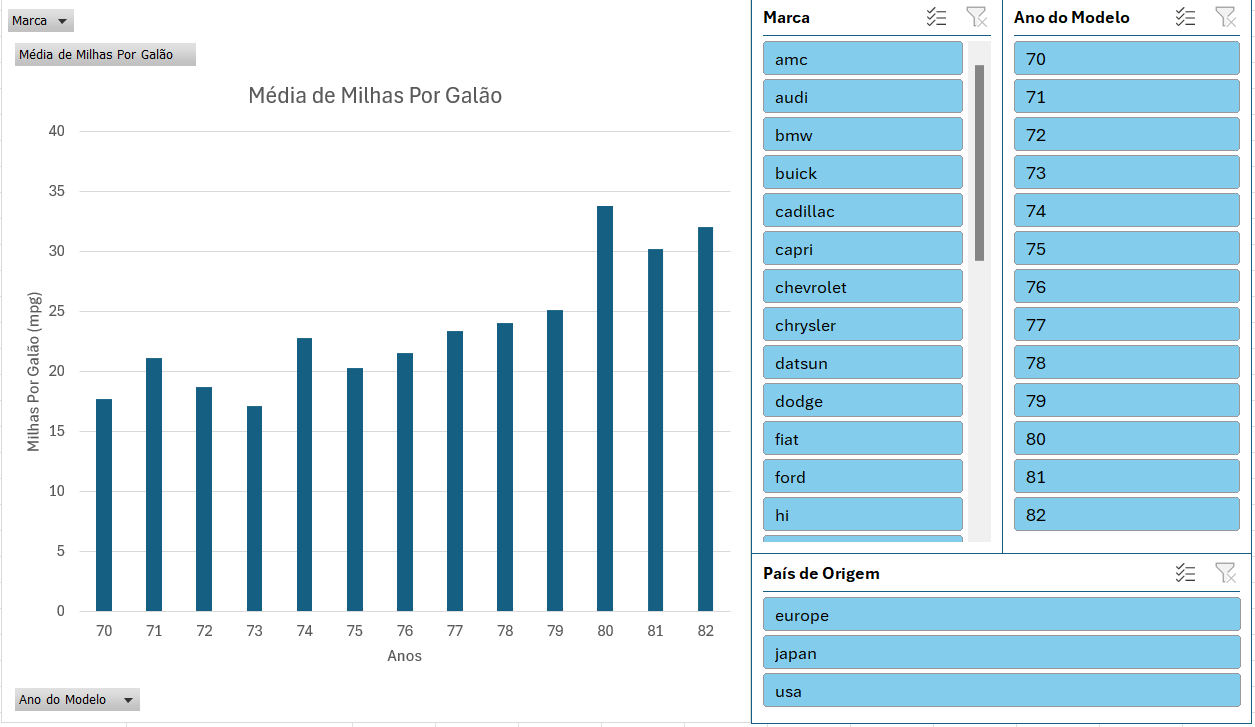
\includegraphics[width=1.2\textwidth]{Recursos/MilhasPorGalaoGrafico.png} % Substitua pelo caminho da imagem
    \vspace{0.5cm}
    \label{fig:mpg}
    \caption{Milhas por galão ao longo dos anos}
\end{figure}
\newpage


%---------------------------------------------------------------------------------------------------------------------------

\subsubsection{Cavalagem}
É possível verificar que a cavalagem dos carros tem diminuido ao longo dos anos, sendo esse um dos motivos
que influenciou a melhoria da eficiência dos carros, pois quanto maior a cavalagem maior o consumo de combustível.
Em 1970 a cavalagem média era de cerca de 150 cavalos e em 1982 a cavalagem média era de cerca de 80 cavalos.
É uma diminuição significativa, que mostra que os carros têm vindo a ser produzidos com motores mais eficientes em termos
de eficiência de combustível, porém sacrificando a sua velocidade e aceleração.

\begin{figure}[h!]
    \centering
    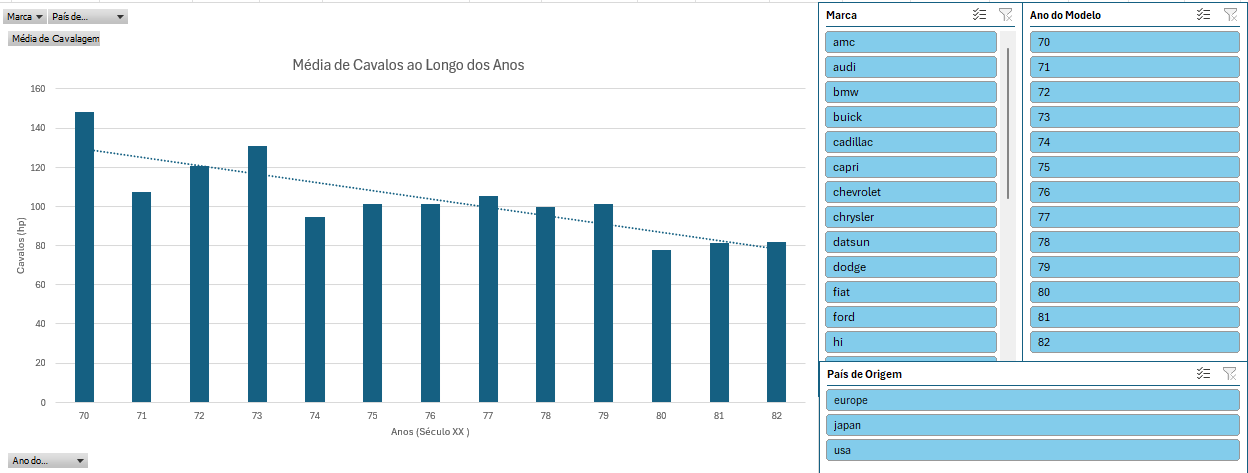
\includegraphics[width=1\textwidth]{Recursos/CavalagemGrafico.png} % Substitua pelo caminho da imagem
    \vspace{0.5cm}
    \label{fig:cavg}
    \caption{Cavalagem ao longo dos anos}
\end{figure}

\newpage
%---------------------------------------------------------------------------------------------------------------------------
\subsubsection{Aceleração Média}
É possível verificar que com a diminuição da cavalagem, o tempo de aceleração dos 0 às 60 milhas por hora dos carros tem vindo a 
aumentar ao longo dos anos, sendo que em 1970 o tempo médio era de cerca de 13 segundos e em 1982 o tempo médio
era de cerca de 16 segundos.
\begin{figure}[h!]
    \centering
    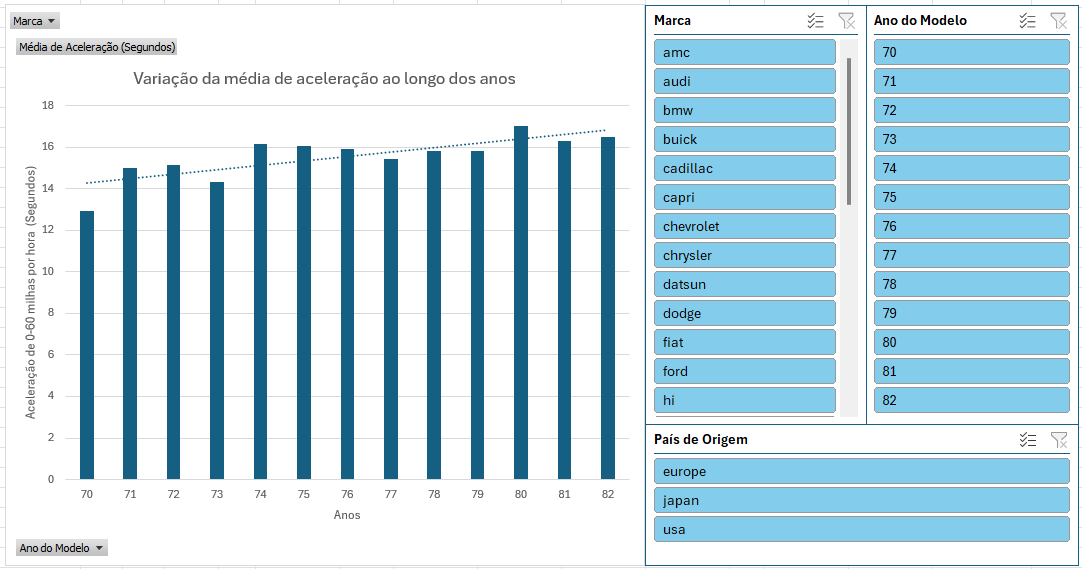
\includegraphics[width=1\textwidth]{Recursos/AceleraçãoMediaGrafico.png} % Substitua pelo caminho da imagem
    \vspace{0.5cm}
    \label{fig:accmg}
    \caption{Aceleração ao longo dos anos}
\end{figure}
\newpage
%---------------------------------------------------------------------------------------------------------------------------
\subsubsection{Número de Veículos}
No gráfico é possível verificar que o número de veículos tem estado estável ao longo dos anos, apesar de 
algumas oscilações, mostrando que o setor automóvel conseguiu adaptar-se à crise do petróleo e manter a produção
de veículos estável. Algumas marcas aumentaram a sua produção, enquanto outras diminuiram.
No entanto, algumas marcas surgiram e outras desapareceram, mostrando que o setor automóvel é muito dinâmico e
está sempre a mudar.

\begin{figure}[h!]
    \centering
    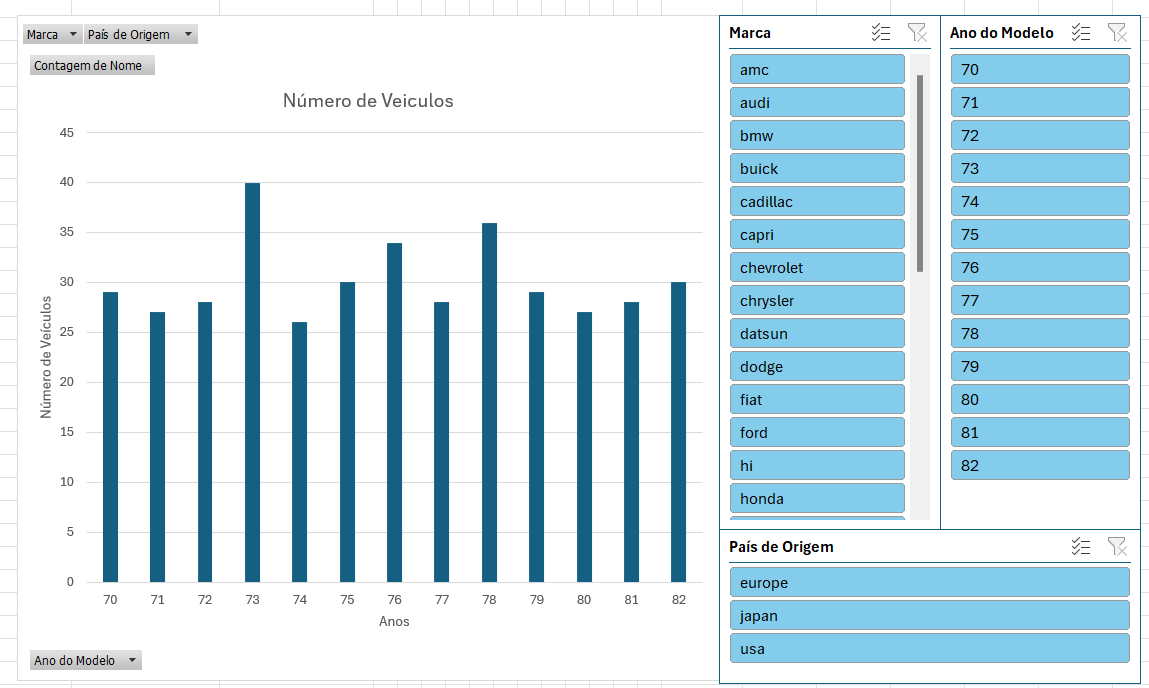
\includegraphics[width=1\textwidth]{Recursos/NVeiculosGrafico.png} % Substitua pelo caminho da imagem
    \vspace{0.5cm}
    \label{fig:nveig}
    \caption{Número de veículos ao longo dos anos}
\end{figure}
\newpage
%---------------------------------------------------------------------------------------------------------------------------
\section{Criação da Dataware House}\label{dwh}
Esta é a nossa proposta de uma Data Warehouse para dada a nossa análise dos dados.

\begin{figure}[h!]
    \centering
    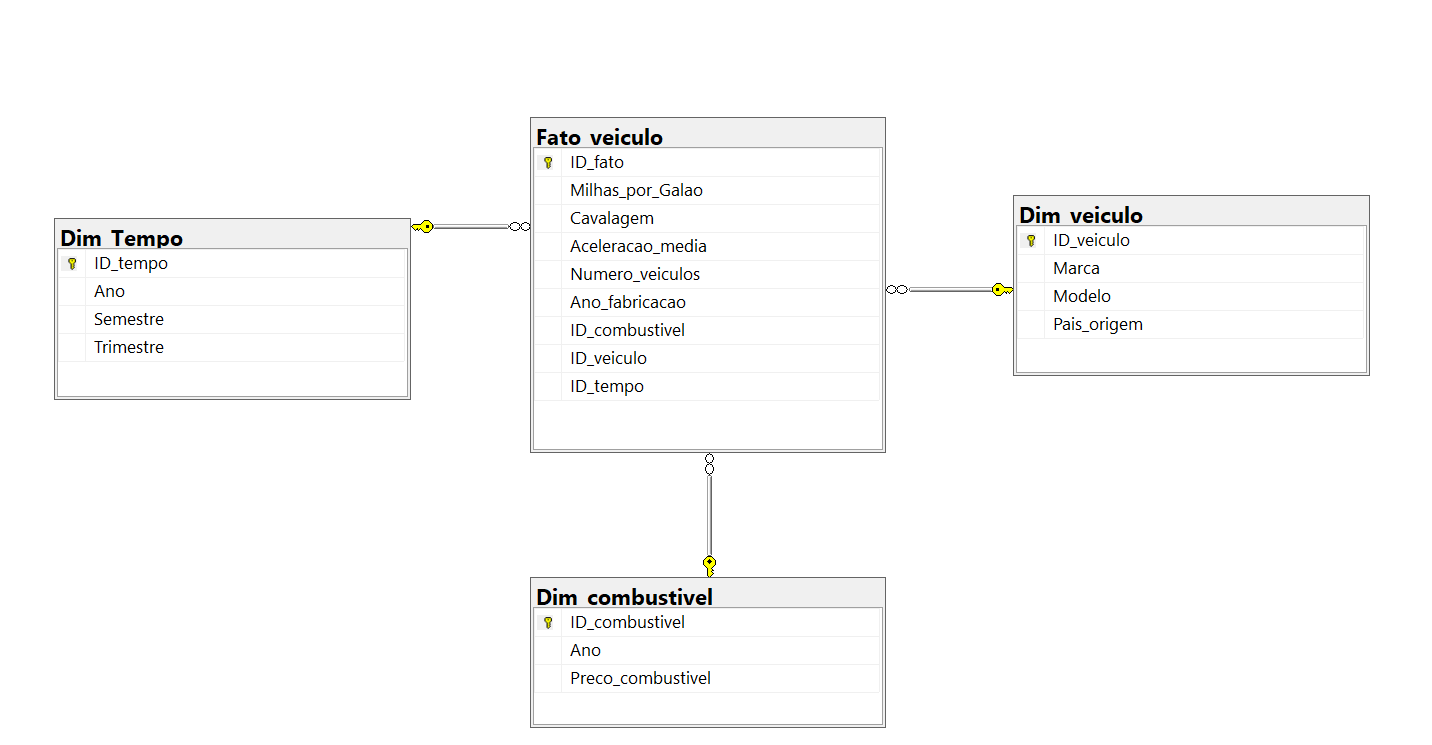
\includegraphics[width=1\textwidth]{Recursos/DiagramaCrisePetroleo.png} % Substitua pelo caminho da imagem
    \vspace{0.5cm}
    \label{fig:dcri}
    \caption{Diagrama da Data Warehouse}
\end{figure}
\newpage
%---------------------------------------------------------------------------------------------------------------------------
\section{Contexto Global}\label{cg}
As Crises Petrolíferas de 1973 e 1979 dão contexto às mudanças drasticas nos automóveis que foram visualizadas anteriormente.

A Crise Petrolífera de 1973 (\cite{pet73}) teve início em outubro de 1973 quando os membros da 
Organização dos Países Árabes Exportadores de Petróleo (OPAEP), que compreende os membros árabes da 
Organização dos Países Exportadores de Petróleo (OPEP), além do Egito e Síria, proclamaram um embargo petrolífero. 
O embargo foi direcionado as nações que eram vistas como apoiantes de Israel durante a Guerra do Yom Kippur. 
As nações alvo do embargo foram inicialmente o Canadá, o Japão, a Holanda, o Reino Unido e os Estados Unidos, 
com o embargo também mais tarde a expandir-se para Portugal, Rodésia e África do Sul. Até o fim do embargo, em março de 1974, 
o preço do petróleo subiu de 3 dólares por barril para cerca de 12 dólares no mundo inteiro. Os preços nos EUA foram ainda mais altos. 
O embargo causou uma crise, ou "choque" de petróleo, com muitos efeitos, de curto ou longo prazo, na política e economia global. 
Mais tarde, foi chamada o "primeiro choque do petróleo", seguido pela crise do petróleo de 1979, chamada o "segundo choque do petróleo."

A Crise Petrolífera de 1979 (\cite{pet79}) ocorreu no mundo devido à diminuição da produção de petróleo após a Revolução Iraniana. 
Apesar das reservas globais de petróleo terem diminuido pouco, o pânico generalizado resultou em uma elevação brusca do preço, 
que aumentou para 39,50 dólares por barril nos 12 meses seguintes, o que formou longas filas em postos de gasolina, como na crise petrolífera de 1973.

Estas Crises Petrolíferas fizeram com que os fabricantes de automóveis tivessem de se adaptar e produzir carros mais eficientes, estas adaptações para 
veiculos americanos foram dificeis, cujos quais eram conhecidos por serem grandes e terem motores grandes que gastam muito combustível,
tiveram a sua potencia drasticamente diminuida ao ponto dos modelos desportivos serem considerados muito lentos para a sua categoria.
Os japoneses aproveitaram a situação pois já produziam carros mais pequenos e eficientes e decidiram começar a vender mais no mercado americano,
aumentando a sua quota de mercado significativamente.
%---------------------------------------------------------------------------------------------------------------------------

\newpage
\renewcommand{\refname}{Bibliografia} % Para artigos
\renewcommand{\bibname}{Bibliografia} % Para livros e relatórios
\addcontentsline{toc}{section}{Bibliografia} % Adiciona a Bibliografia ao índice
\printbibliography

\end{document}
